\documentclass[titlepage]{article}
\usepackage{totpages}
\def\CurrentOption{} % fix bug in totpages
\usepackage{sf298}
\usepackage{pgfgantt}
\usepackage{graphicx}
\usepackage{fullpage}
\usepackage{amsmath}

\usepackage[T1]{fontenc}
\usepackage[utf8]{luainputenc}
\usepackage{geometry}
\geometry{verbose,tmargin=1in,bmargin=1in,lmargin=1in,rmargin=1in}
\usepackage{float}
\usepackage{amsbsy}
\usepackage{stackrel}
%\usepackage{subfig}
\usepackage{subfigure}[1995/03/06]
\usepackage{esint}
\usepackage{enumitem}
\usepackage{algorithm}
\usepackage[noend]{algpseudocode}
\usepackage{pdfpages}
\DeclareGraphicsExtensions{.png}
\usepackage{enumitem}
\setlist[description]{leftmargin=\parindent,labelindent=\parindent}

\definecolor{wwwwww}{rgb}{0.4,0.4,0.4}
\definecolor{qqwwww}{rgb}{0,0.4,0.4}
\definecolor{qqzzzz}{rgb}{0,0.6,0.6}

\newlength{\sspace}
\setlength{\sspace}{-0.8em}

\newlength{\cspace}
\setlength{\cspace}{-3.0em}

\newlength{\capwidth}
\setlength{\capwidth}{5.5in}

\title{{\tt CAPS}: \\ Computational Aircraft Prototype Syntheses \\ ~ \\ \Large Monthly Report -- February 2018\\[0.04in]
% \large and \\ \Large Annual Report -- Year \#1
}
\author{Robert Haimes, PI \\ John F. Dannenhoffer, III
\\ Julia Docampo-S\'anchez
%\\ Mark Drela 
%\\ Marshall C. Galbraith 
%\\ Philip Caplan
%\\ Steven R. Allmaras
%\\ David Marcum
%\\Steve Karman
}

%                  DD MM YYYY
\ReportDate{yy--03--2018}
\ReportType{Technical Report}
\DatesCovered{1 February 2018 -- 28 February 2018}
\Title{{\tt CAPS} Monthly Status Report}
\ContractNumber{FA8650--14--C--2472}
\Author{Haimes, Robert
%\\Drela, Mark
%\\ Galbraith, Marshall , C.
%\\Caplan, Philip
\\ Docampo-S\'anchez, Julia
\\ Dannenhoffer, John, F, III*
%\\Marcum, David**
%\\Karman, Steve$\dagger$
}
\PerformingOrg{MIT, Cambridge MA \\ Syracuse University, Syracuse NY* %\\ Mississippi State University, Starkville MS**
%\\Pointwise, Inc$\dagger$
}
\SponsoringAgency{Air Force Research Labs \\ Wright-Patterson AFB, OH}
\Acronyms{AFRL/RQVC}
\SMReportNumber{Data Item No. A006}
\Abstract{The objective of this effort is to establish a computational geometry, meshing and analysis model generation tool that can be used across AFRL/RQV. This common tool will enable collaboration between conceptual design, multidisciplinary optimization and high fidelity simulation efforts.}
\SubjectTerms{multidisciplinary analysis; multi-fidelity geometry; aircraft design; software infrastructure}
\AbstractLimitation{UU}
\ResponsiblePerson{Robert Haimes}
\RPTelephone{(617) 253--7518}

\NumberPages{xx}

\begin{document}

\bibliographystyle{unsrt}

  \maketitle

  \MakeRptDocPage
  
%    \tableofcontents

\newpage
  \section{Combined Operations}
  Although a swap, collapse or split alone may not be able to produce a regular region,  we can 
  combine these operations in order to reduce the total number of irregular vertices. We 
  achieve this by looking at several vertex stars and bringing together (closer) irregular vertices. 
   In general, if there are only two irregular vertices nearby, 
   $e.g.$ a quad with two vertices with valence three, then a collapse would convert those vertices 
   into a regular vertex but produce two new valence three vertices. Similarly, if we swap a (5,5) vertex 
   pair with  a (4,4) pair, overall, we have not improved. However, in both cases, we have changed 
   the location of the irregular vertices. Thus, if there is a third vertex with high/low valence in the 
   neighborhood, now there are three irregular vertices together and we can improve the mesh quality. 
   
   We will show next the following combined operations: swap and split, split and collapse and double split. 
  
  \section {Irregular Quads}
  Once the basic operations can no longer improve the overall quality, rather than looking at vertices, 
  we now turn our attention towards the quads and look for cases where we have (3,5,5,4) valences. 
  Notice that swapping is effective only if there are irregular vertices with two adjacent quads but 
  not when all the vertices belong to the same quad. Ideally, we want to avoid collapsing as much as possible since 
  this would lead to mesh coarsening. Therefore, initially, we will only pair a collapse ( -1 vertex) 
  with a split ( +1 vertex) so that the number of vertices remains unaltered. 
  
  
  
  
  
 \subsection{Collapse And Split} 
  If we have a quad with vertices (3,4,5,5), $i.e.$, the valence three is opposite to the valence five, 
  then we can collapse this pair, producing temporarily a (3,6,4) link as shown in Figure \ref{fig:collapse_and_split_1}. 
  Now, we can split the  6 valence using the vertex with valence 3 which will produce either a full regular region 
  or only add a valence to the opposite vertex (see Figure \ref{fig:collapse_and_split_2}). Overall, we have
   gone from 3 irregular vertices to one (zero). 
   
   
   
   
  The swap and split operation is effective when we have a quad with three irregular vertices (3,5,5,4). 
  belong to the same quad. two valence 5 pairs belong to the same quad and 
  there is a valence 3 vertex connected to one of them. Then, by within the star range of one of the other two vertices. 



  \subsection{Swap And Split } 
  
  During the first scans, we ensure that all the higher valence (6+) vertices are reduced so that we are 
  only left with either valences 3,4 or 5. 
  The swap and split operation is effective when we have a quad with three irregular vertices (3,5,5,4). 
  belong to the same quad. two valence 5 pairs belong to the same quad and 
  there is a valence 3 vertex connected to one of them. Then, by within the star range of one of the other two vertices. 
  
  
  
  
  
  
  
  
  
  
  
   \begin{figure}
  \centering
 \begin{tabular}{cccc}
 Original & Basic & Combined & Optimized\\
\scalebox{0.45}{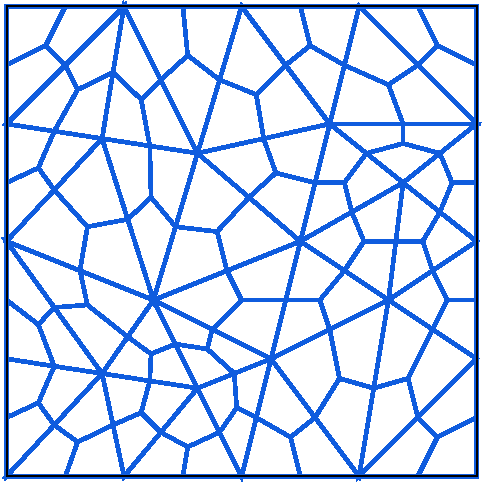
\includegraphics{PLOTS/init.pdf}}&
\scalebox{0.45}{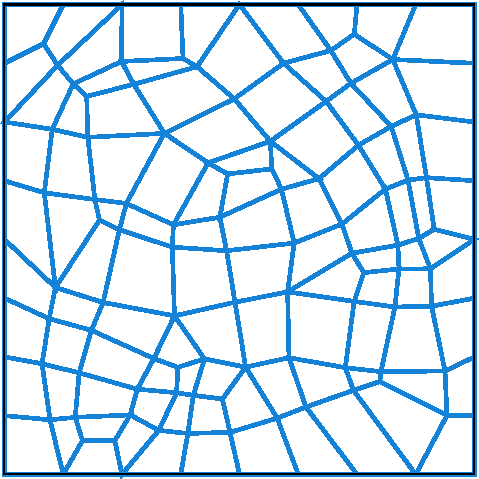
\includegraphics{PLOTS/noswapsplit.pdf}}&
\scalebox{0.45}{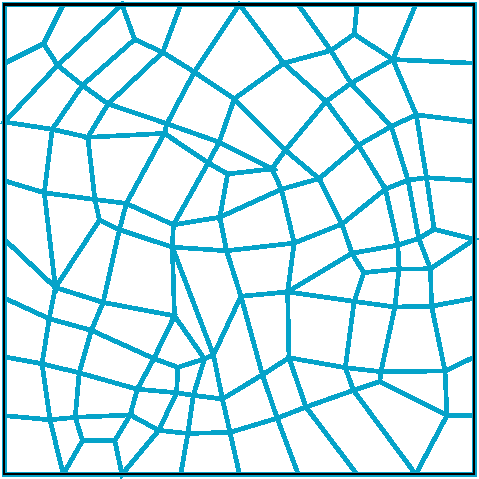
\includegraphics{PLOTS/swapsplit.pdf}}&
\scalebox{0.45}{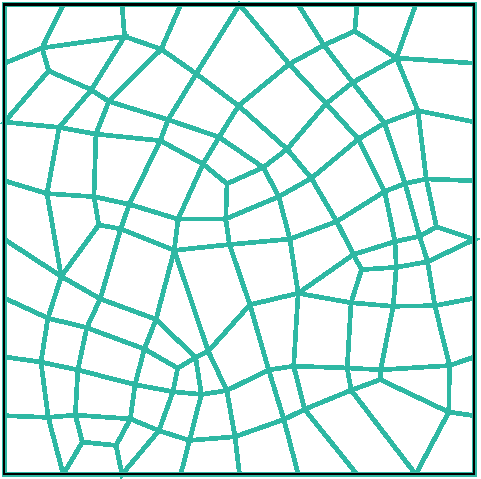
\includegraphics{PLOTS/optimized.pdf}}
 \end{tabular}
 \caption{Illustration of the regularization process showing the initial mesh (left), the single element operation process (second image), 
  further regularization by combining swap\&split and the final mesh afer being optimized (right.}
 \label{fig:invalid_quad}
 \end{figure}
  
  
  \begin{figure}
  \centering
 \begin{tabular}{cc}
  Overlap &  Zooming into one region\\
\scalebox{0.6}{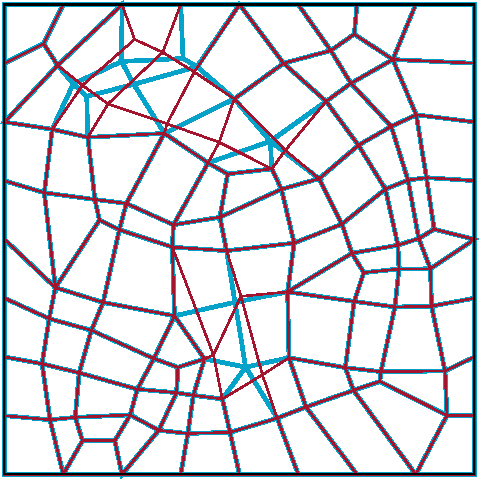
\includegraphics{PLOTS/overlap2.pdf}}&
\scalebox{0.6}{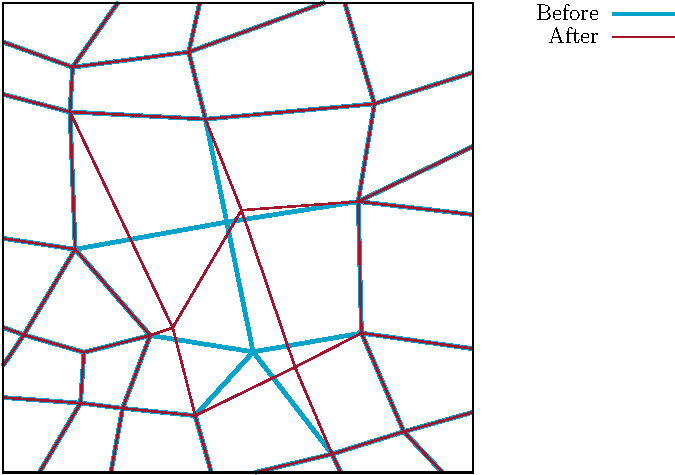
\includegraphics{PLOTS/overlapZOOM.pdf}}
 \end{tabular}
 \caption{Swap\&split operation: the left plot shows all the places where we could apply the technique and the 
 right plot is a zoom of the lower swap and split step showing how we have gone from three irregular vertices (2 valence 5, 1 valence 3) to 1 irregular vertex (valence 5). }
 \label{fig:invalid_quad}
 \end{figure}
  
  
  
  
  
  
  
  
  
  
  
  
  
  
  
  \section{Curvature Driven Element Sizing}
  Let $K_1$ and $K_2$ denote the principal curvatures and $\vec k_1, \vec k_2$ the principal directions. 
  We will cast the optimization problem based on the surface curvature in the following way: reallocate the vertices so that they are 
  aligned with the principal directions and the edge size reflects the underlying curvature. 
  
 \begin{enumerate}
  \item Element Orientation. During the local (global) optimization process, we combine the equi-angle approach with 
  the principal curvature directions; for irregular vertices (valence $\neq$ 4), since we cannot align with the curvature directions (two directions = four edges) we compute the error assuming that the 
  optimal distribution will produce equal internal angles. On the other hand, for regular vertices, we proceed as follows. At each vertex:
  \begin{itemize}
   \item Get principal directions.
   \item Construct normal plane to the surface. 
   \item Project each of the linking vertices (edges) onto the normal plane. 
   \item Find the edge that is closest to any of the curvature directions (pivot). 
   \item Compute the four angles using the pivot as leading direction. 
  \end{itemize}
  Figure \ref{} illustrates this operation. 
At each vertex we obtain the principal directions and construct the normal plane. 
 

 
 
\begin{figure}
\centering
\definecolor{qqwuqq}{rgb}{0,0.39,0}
\definecolor{ffqqqq}{rgb}{1,0,0}
\definecolor{cccccc}{rgb}{0.8,0.8,0.8}
\definecolor{qqqqff}{rgb}{0,0,1}
\begin{tikzpicture}[line cap=round,line join=round,>=triangle 45,x=1.0cm,y=1.0cm]
\clip(1.54,11.96) rectangle (12.7,19.7);
\fill[color=cccccc,fill=cccccc,fill opacity=0.5] (5.71,18.31) -- (8.22,19.43) -- (9.76,15.99) -- (7.25,14.87) -- cycle;
\draw [shift={(7.8,16.98)},line width=1.2pt,color=ffqqqq,fill=ffqqqq,fill opacity=0.75] (0,0) -- (-155.92:0.6) arc (-155.92:-137.12:0.6) -- cycle;
\draw [shift={(7.8,16.98)},color=qqwuqq,fill=qqwuqq,fill opacity=0.1] (0,0) -- (-65.92:0.6) arc (-65.92:-26.19:0.6) -- cycle;
\draw [shift={(7.8,16.98)},color=qqwuqq,fill=qqwuqq,fill opacity=0.1] (0,0) -- (24.08:0.6) arc (24.08:61.03:0.6) -- cycle;
\draw [shift={(7.8,16.98)},color=qqwuqq,fill=qqwuqq,fill opacity=0.1] (0,0) -- (114.08:0.6) arc (114.08:165.96:0.6) -- cycle;
\draw [shift={(3.4,14.46)}] plot[domain=-0.31:1.88,variable=\t]({1*2.65*cos(\t r)+0*2.65*sin(\t r)},{0*2.65*cos(\t r)+1*2.65*sin(\t r)});
\draw (5.92,13.64)-- (11.28,16.04);
\draw (2.63,17)-- (8.32,18.85);
\draw [shift={(8.46,16.02)}] plot[domain=0.01:1.62,variable=\t]({1*2.82*cos(\t r)+0*2.82*sin(\t r)},{0*2.82*cos(\t r)+1*2.82*sin(\t r)});
\draw [color=cccccc] (5.71,18.31)-- (8.22,19.43);
\draw [color=cccccc] (8.22,19.43)-- (9.76,15.99);
\draw [color=cccccc] (9.76,15.99)-- (7.25,14.87);
\draw [color=cccccc] (7.25,14.87)-- (5.71,18.31);
\draw [->] (7.8,16.98) -- (9.07,17.55);
\draw [->] (7.8,16.98) -- (6.96,18.87);
\draw [->] (7.8,16.98) -- (8.49,15.43);
\draw [->] (7.8,16.98) -- (6.56,16.42);
\draw (7.8,16.98)-- (8.42,18.1);
\draw (7.8,16.98)-- (6.52,17.3);
\draw (7.8,16.98)-- (6.96,16.2);
\draw (7.8,16.98)-- (9.02,16.38);
\begin{scriptsize}
\fill [color=qqqqff] (7.8,16.98) circle (1.5pt);
\fill [color=qqqqff] (8.42,18.1) circle (1.5pt);
\fill [color=qqqqff] (6.52,17.3) circle (1.5pt);
\fill [color=qqqqff] (6.96,16.2) circle (1.5pt);
\fill [color=qqqqff] (9.02,16.38) circle (1.5pt);
\end{scriptsize}
\end{tikzpicture}
\caption{\label{fig:} }
\end{figure}
  
  
  
 
  
  
  
  
  
  \item Element Size. We use an approach suggested in []. From any vertex, we compute a metric based on the local curvature approximating the arc-length by the chord: 
  \begin{align}
   s &= \frac{\ell}{ 1- \epsilon}\\
   g(\epsilon) &= \sqrt{40(1-(\sqrt{1-1.2\epsilon)}}
  \end{align}
  where $s$ denotes the arc-length, $\ell$ the chord and $\epsilon$ is a user defined tolerance. This equation is obtained by 
   linearization, using that $s= c\theta$, being $c$ the radius of curvature and $\theta$ the angle with respect the principal curvature. 

  \end{enumerate}
  
  
  
  
  
  
  \end{document}
  
  